        %%%%%%%%%%%%%%%%%%%%%%%%%%%%%%%%%%%%%%%%%%%%%%%%%%%%%%%%%%%%%%%%%%%%%%%%%%%%%%%%%%%%
%Do not alter this block of commands.  If you're proficient at LaTeX, you may include additional packages, create macros, etc. immediately below this block of commands, but make sure to NOT alter the header, margin, and comment settings here. 
\documentclass[12pt]{article}
 \usepackage[margin=1in]{geometry} 
\usepackage{amsmath,amsthm,amssymb,amsfonts, enumitem, fancyhdr, color, hyperref,comment, graphicx, environ,mathtools, bbm, tikz, setspace, cleveref,listings, dcolumn}
\usepackage{array, multirow, caption, booktabs}
\usepackage{ mathrsfs }
\usetikzlibrary{matrix,positioning}
\tikzset{bullet/.style={circle,draw=black,inner sep=8pt}}
\DeclareMathOperator*{\argmax}{arg\,max}
\DeclareMathOperator*{\argmin}{arg\,min}
\DeclareMathOperator*{\Var}{\text{Var}}
\DeclareMathOperator*{\Cov}{\text{Cov}}

\DeclarePairedDelimiter\norm{\lVert}{\rVert}%
\newtheorem{theorem}{Theorem}
\newtheorem{lemma}[theorem]{Lemma}
\DeclareMathOperator{\eps}{\varepsilon}
\doublespacing
\DeclarePairedDelimiter\abs{\lvert}{\rvert}%
\pagestyle{fancy}
\setlength{\headheight}{65pt}
\newenvironment{problem}[2][Problem]{\begin{trivlist}
\item[\hskip \labelsep {\bfseries #1}\hskip \labelsep {\bfseries #2.}]}{\end{trivlist}}
\newenvironment{sol}
    {\emph{Solution:}
    }
    {
    \qed
    }


%%%%%%%%%%%%%%%%%%%%%%%%%%%%%%%%%%%%%%%%%%%%%%%%%%%%%%%%%%%%%%%%%%%%%%%%%%%%%%%%%


\usepackage{xcolor}
 
 


%%%%%%%%%%%%%%%%%%%%%%%%%%%%%%%%%%%%%%%%%%%%%

\rhead{Asha Bharadwaj, Caitlin Dutta, John Higgins, Alexis Smith\\Econ 899 \\ 21 September, 2022} 

%%%%%%%%%%%%%%%%%%%%%%%%%%%%%%%%%%%%%%%%%%%%%


%%%%%%%%%%%%%%%%%%%%%%%%%%%%%%%%%%%%%%

\begin{document}

\section{I. Huggett (1993) with enforceable insurance}
As in Hugget (1993), suppose there is a continuum of agents with total mass equal to one. Each agent has no initial asset holdings. Each period, agents receive an endowment of a consumption good. The endowment $e$ takes values in $E = \{e_h, e_l\}$, with $e_h > e_l$. 

The endowment process for each agent follows a Markov process with $\pi(e' \mid e) = P(e_{t+1} = e' \mid e_{t} = e) > 0$ for each $e, e' \in E$. We assume each realization of the endowment process is iid and thus independent of all other agents' endowment realizations.

Agents have preferences given by 
\[E\left[ \sum_{t=0}^{\infty} \beta^t \frac{c^{1-\sigma}}{1-\sigma}\right] \quad \sigma > 1\]
where $E$ is the expectation operator with respect to the stochastic endowment process.

Agents are able to purchase state-contingent insurance which pays out based on their realization of their endowment in the next period. That is, agents can buy and sell Arrow securities $a_h^{t+1}$ and $a_l^{t+1}$, where $a_h^{t+1}$ pays out one unit of the consumption good in period $t+1$ when the agent receives endowment $e_h$, and $a_l^{t+1}$ pays out one unit when the agent receives $e_l$. These time $t$ contracts have prices $q_h^{t}$ and $q_l^{t}$, respectively. We assume these contracts are enforceable and thus all agents can credibly commit to fulfilling their obligations.

Agents in time $t$ with current endowment $e_h$ and current holdings $a_h^t$ and $a_l^t$ facing prices $q_h^t$ and $q_l^t$ obey the following constraint:
\[c_t + q_l^t a_l^{t+1} + q_h^t a_h^{t+1} \leq e_h + a_h^t\]
Similarly, agents with endowment $e_l$ have the following constraint:
\[c_t + q_l^t a_l^{t+1} + q_h^t a_h^{t+1} \leq e_l + a_l^t\]
Now that we have set up the problem, we wish to find the competitive equilibrium of such an economy. We start by finding the solution to the planner's problem and then decentralizing it.

Let $\Pi_h^t$ and $\Pi_l^{t}$ indicate the proportion of agents in time $t$ with $e_h$ and $e_l$, respectively. %Since there is a continuum of agents which each realize iid endowment shocks, the Law of Large Numbers dictates that the proportion of agents with endowment $e_h$ will simply be $\Pi_h^{t+1} = \pi(e_h \mid e_h) \Pi_h^{t} + \pi(e_h \mid e_l) \Pi_l^t$. Similarly, the mass of agents with endowment $e_l$ will be $

Assuming the planner is utilitarian and weighs all agents equally, the planner solves
\begin{align*}
    \max_{\{c_h^t, c_l^t\}_{t=0}^{\infty}} \sum_{t=0}^{\infty} \beta^t \left[\Pi_h^t \frac{(c_h^t)^{1-\sigma}}{1-\sigma} + \Pi_l^t \frac{(c_l^t)^{1-\sigma}}{1-\sigma} \right] \\
    \text{s.t. } c_h^t, c_h^t \geq 0, \quad \forall t\\
    \Pi_h^t c_h^t + \Pi_l^t c_l^t \leq \Pi_h^t e_h + \Pi_l^t e_l, \quad \forall t
\end{align*}
Assuming the non-negativity constraint on consumption doesn't bind, the planner's problem has the following Lagrangian:
\[\mathcal{L} = \sum_{t=0}^{\infty} \beta^t \left[\Pi_h^t \frac{(c_h^t)^{1-\sigma}}{1-\sigma} + \Pi_l^t \frac{(c_l^t)^{1-\sigma}}{1-\sigma} \right] + \lambda_t [\Pi_h^t e_h + \Pi_l^t e_l - \Pi_h^t c_h^t - \Pi_l^t c_l^t]\]
This has the following first order conditions:
\[\beta^t \Pi_h^t (c_h^t)^{-\sigma}  \leq \Pi_h^t \lambda_t \]
\[\beta^t \Pi_l^t (c_l^t)^{-\sigma} \leq \Pi_l^t \lambda_t \]
with $\lambda_t \geq 0$ $\forall t$, as well as the complementary slackness condition:
\[\lambda_t[\Pi_h^t e_h + \Pi_l^t e_l - \Pi_h^t c_h^t - \Pi_l^t c_l^t] = 0\]
If we let the inequality constraints bind, we note that we have
\[(c_h^t)^{-\sigma} =( c_l^t)^{-\sigma} = \lambda_t > 0\]
since $c_h^t, c_l^t >0$ by our initial assumption. This means that the planner will optimally set $c_h^t = c_l^t = c^t$ $\forall t$. It now remains to find $c^t$. Note that since $\lambda_t > 0$ $\forall t$, it follows that the planner's resource constraint will bind. Hence,
\[\Pi_h^t c^t + \Pi_l^t c^t = \Pi_h^t e_h + \Pi_l^t e_l \iff c^t = \frac{\Pi_h^t e_h + \Pi_l^t e_l}{\Pi_h^t + \Pi_l^t} =\Pi_h^t e_h + \Pi_l^t e_l \]
since $\Pi_h^t + \Pi_l^t = 1$.  

Furthermore, if the Markov process is assumed to have a stationary distribution, we note that $\Pi_h^t = \Pi_h$ and $\Pi_l^t = \Pi_l$ for all $t$, for some $\Pi_h$ and $\Pi_l$ such that $\Pi_h + \Pi_l = 1$ (since there is a continuum of agents). This means that the allocation is constant across time (since the aggregate endowment is constant). Therefore, we have that 
\[\forall t, c^t = \bar{c} = \Pi_h e_h + \Pi_l e_l\]

In summary, the planner sets consumption for all agents to be the same, and the allocation depends only on the aggregate endowment which is constant across time. 

For concreteness, we use the parameterization specified in part II which has $e_h = 1$, $e_l = 0.5$, $\Pi_l = 0.0566$, and $\Pi_h = 0.9434$. Hence,
\[\bar{c} = 0.9434 \cdot 1 + 0.0566 \cdot 0.5 = 0.9717\]

We now decentralize this solution using the Arrow-security setup specified previously. A competitive equilibrium involves agents maximizing their utility as described above and markets clearing. We note that, in order to implement the planner's solution, it must be the case that agents sell $a_h^{t+1}$ and buy $a_l^{t+1}$ to insure themselves against adverse shocks (since $e_l < \bar{c} < e_h$).

Let $c(e_t)$ indicate the consumption of an agent with endowment $e_t$, and $a(e_t)$ indicate their insurance purchase. The asset market clearing condition is that $\Pi_h a(e_h) = -\Pi_l a(e_l)$.

The agent's problem is thus
\[\max_{c(e_t), a(e_{t+1})} E\left[ \sum_{t=0}^{\infty} \frac{c(e_t)^{1-\sigma}}{1-\sigma}\right]\]
subject to the sequential budget constraint
\[c(e_t) + q a(e_{t+1}) \leq e_t + a(e_t)\]
Their Lagrangian is the following:
\[\mathcal{L} = E\left[\sum_{t=0}^{\infty} \beta^t\frac{c(e_t)^{1-\sigma}}{1-\sigma}\right] + \lambda_t [ e_t + a(e_{t+1}) - c(e_t) - q a(e_t)]\]
which has FOCs
\[\beta^t c(e_t)^{-\sigma} =\lambda_t \quad [c(e_t)]\]
\[\lambda_t = q \lambda_{t+1} \quad [a(e_{t+1})]\]
Combining these, we obtain
\[\beta^t c(e_t)^{-\sigma} = q \beta^{t+1} c(e_{t+1})^{-\sigma}\]
Imposing the condition from the planner's allocation that $c(e_t) = c(e_{t+1}) = \bar{c}$ $\forall t$, it follows that
\[\beta^t = q \beta^{t+1} \implies q = \beta\]
Hence, the price to a claim on consumption in the next period is given by $q= \beta$. The allocation of consumption is the same as the planner's problem. It remains to find the assets purchased by each type. We note that
\[a(e_h) = \bar{c} - e_h \quad \text{and} \quad a(e_l) = \bar{c} - e_l\]
Again using the parameterization from part II, this implies that
\[a(e_h) = -0.0283 \quad \text{and} \quad a(e_l) = 0.4717\]
We verify that asset market clearing is satisfied:
\[\Pi_h a(e_h) =(0.9434) (-0.0283) = -0.0267 = -(0.0566)(0.4717) = -\Pi_l a(e_l) \]
\section{II. Computing Huggett with incomplete markets} 
\begin{enumerate}[label=\alph*) ]
    \item The plot of the policy function $g(a,s)$ for each $s$ is included below, alongside a plot of the 45-degree line.
    \begin{center}
        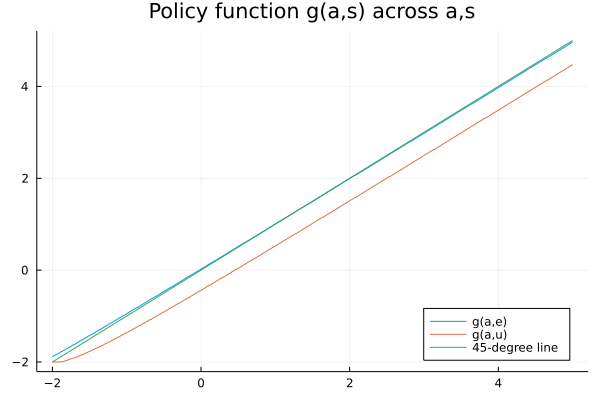
\includegraphics[scale=0.5]{pfplot.png}
    \end{center}
    To verify that $\exists \hat{a}$ such that $g(\hat{a}, s) < \hat{a}$, we plot $g(a, s) - a$ for each $(a,s)$ combination in the following figure:
    \begin{center}
        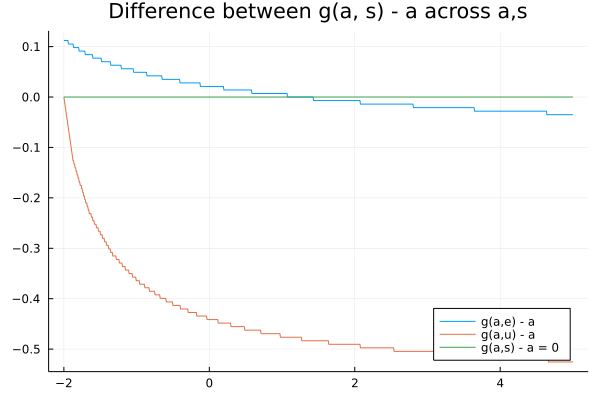
\includegraphics[scale=0.5]{pfdiffplot.png}
    \end{center}
    The first $a$ such that $g(a, s) \leq a$ is given by $\hat{a} \approx 1.076$ for employed agents and $\hat{a} =-2$ for unemployed agents.
    \item The market-clearing bond price is approximately 0.99427. The stationary cross-sectional distribution associated with this price is plotted below:
    \begin{center}
        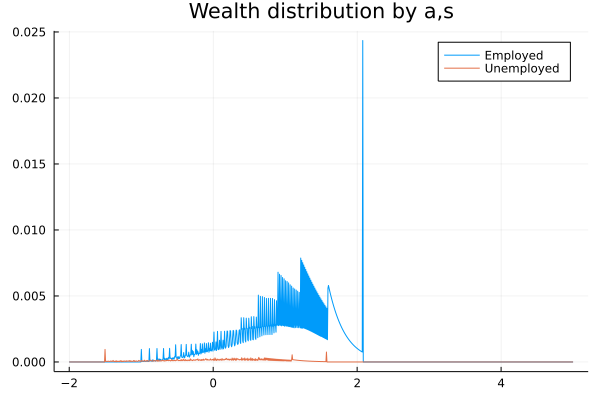
\includegraphics[scale=0.5]{wealthplot.png}
    \end{center}
    \item The plot of the Lorenz curve is included below. We estimate the gini index to be 0.3843. 
    \begin{center}
        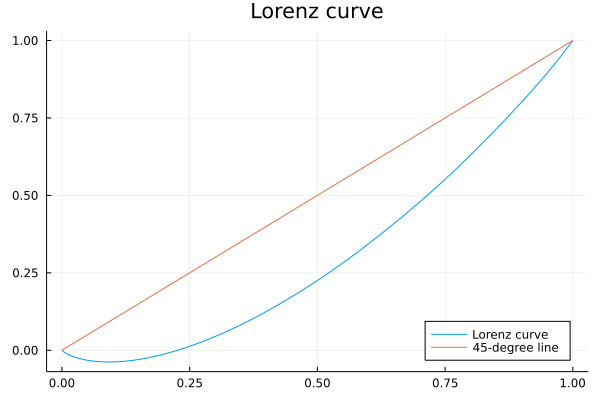
\includegraphics[scale=0.5]{lorenzplot.png}
    \end{center}
    Comparing these with the data, we see that our Lorenz curve is not nearly as curved as the Lorenz curve in the data. As a consequence, our gini coefficient is far less than that computed from the data. The real gini coefficient for wealth is 0.816, whereas ours is less than half of this. This suggests that this model alone cannot account for the degree of inequality observed in the data.
\end{enumerate}
\section{III. Comparing complete and incomplete markets}
    \begin{enumerate}[label=\alph*) ]
        \item We compute the consumption equivalent $\lambda(a, s)$ using the following formula:
        \[\lambda(a,s) = \left[ \frac{W^{FB} + \frac{1}{(1-\alpha)(1-\beta)}}{v(a,s) + \frac{1}{(1-\alpha)(1-\beta)}}\right]^{1/(1-\alpha)} -1\]
        where $W^{FB}$ represent's an agents discounted present value of consumption under the complete markets framework. Given that $c^{FB} = 0.9717$, it follows that
        \[W^{FB} = \sum_{t=0}^{\infty} \beta^t u(0.9717) = \frac{(0.9717)^{1-\alpha} -1}{1-\alpha} \frac{1}{1-\beta} \approx -4.2526\]
        We now compute $\lambda(a,s)$ $\forall a,s$ and plot the curves below for each employment status:
        \begin{center}
            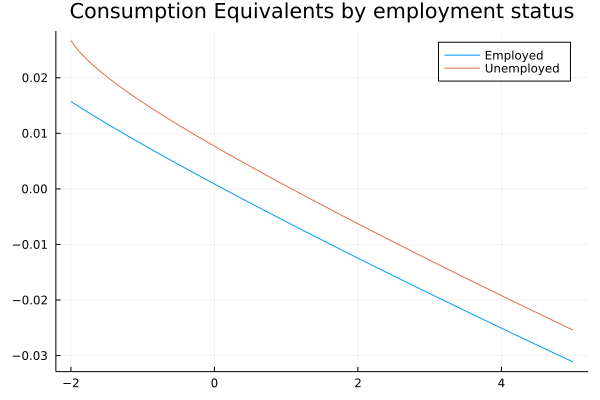
\includegraphics[scale=0.5]{lambdaplot.png}
        \end{center}
        Clearly, unemployed agents are willing to pay more to have access to complete markets because they are not able to smooth consumption in incomplete markets as much as they could with complete markets. Furthermore, agents with lower levels of asset holdings would prefer complete markets because they don't have as much assets on hand to smooth consumption over future shocks. Agents with higher wealth holdings will prefer to keep incomplete markets, since they already have sufficient assets to smooth consumption over future shocks and their consumption would be lower under complete markets. In other words, they would have to give up consumption when going from incomplete to complete markets, so it is understandable why they would not be in favor of switching.
        \item As previously identified, $W^{FB} = -4.2526$. We compute that $W^{INC}= -4.4574$ and $WG = 0.00138$. These indicate that aggregate welfare is lower under incomplete markets, and that the economy-wide welfare gain from complete markets is positive.
        \item The fraction of the population which would prefer changing to complete markets is given by
        \[\sum_{a,s \in A\times S} \mathbbm{1}_{\{\lambda(a,s) \geq 0\}}(a,s) \mu(a,s) \approx 0.5418\]
        That is, 54\% of agents would prefer to change to complete markets. 
    \end{enumerate}    
    

\end{enumerate}
\end{document}
